%-------------------------------------------------------------------------------
% CAPITOLO 17
%-------------------------------------------------------------------------------
\chapter{Lezione 17}
\label{capitolo_17}
\textit{29/04/2025}

\section{Forma generale del modello di Ising}
Il modello di Ising è un modello fondamentale in meccanica statistica. L'Hamiltoniana nella sua forma più generale, che descrive l'energia di una data configurazione di spin $\{S_i\}$, è data da:

\begin{equation} \label{eq:ch17_1}
H = -J \sum_{\langle i,j \rangle} S_i S_j - \sum_i h_i S_i
\end{equation}

Dove:
\begin{itemize}
    \item $S_i$ sono le variabili di spin, che possono assumere i valori $\pm 1$.
    \item La prima somma è estesa a tutte le coppie di spin primi vicini $\langle i,j \rangle$ su un reticolo.
    \item $J$ è la costante di accoppiamento. Se $J>0$, l'interazione è ferromagnetica e gli spin tendono ad allinearsi.
    \item $h_i$ è un campo magnetico esterno che può essere dipendente dal sito $i$.
\end{itemize}

Il termine di interazione può essere riscritto come $\frac{1}{2} \sum_{i \neq j} J_{ij} S_i S_j$, dove $J_{ij}$ è la matrice di interazione.

\section{Approssimazione di Campo Medio (Mean Field)}
Risolvere esattamente questo modello è complesso. Un'approssimazione potente è quella del campo medio. L'idea fisica è che ogni spin non interagisce con lo stato istantaneo dei suoi vicini, ma con il loro campo medio. Stiamo di fatto trascurando le correlazioni tra le fluttuazioni degli spin vicini.

Matematicamente, approssimiamo il termine di interazione:

\begin{equation} \label{eq:ch17_2}
\sum_{\langle i,j \rangle} S_i S_j = \frac{1}{2} \sum_i S_i \left( \sum_{j \in N(i)} S_j \right)
\end{equation}

Nell'approssimazione di campo medio, sostituiamo il valore istantaneo dello spin $S_j$ con il suo valore medio $\langle S_j \rangle$. Questo trasforma un termine fluttuante in uno che descrive l'interazione dello spin $S_i$ con un campo medio efficace generato dai suoi vicini.

L'Hamiltoniana di campo medio ($H_{mf}$) diventa:

\begin{equation} \label{eq:ch17_3}
H_{mf} = -\sum_i S_i h_i^{eff}
\end{equation}

Dove $h_i^{eff}$ è il campo efficace:

\begin{equation} \label{eq:ch17_4}
h_i^{eff} = h_i + J \sum_{j \in N(i)} \langle S_j \rangle
\end{equation}

Questo campo ha due contributi: il campo esterno $h_i$ e il campo medio generato dai vicini.

\subsection*{Caso Omogeneo}
Per semplificare, consideriamo il caso omogeneo in cui il campo esterno è uniforme ($h_i = h$ per ogni $i$) e, per simmetria, la magnetizzazione locale media è la stessa per ogni sito ($\langle S_j \rangle = m$). Se $z$ è il numero di primi vicini, il campo efficace diventa:

\begin{equation} \label{eq:ch17_5}
h^{eff} = h + zJm
\end{equation}

Durante la derivazione dell'Hamiltoniana di campo medio, appare anche un termine aggiuntivo che dipende da $m^2$. Questo termine è costante rispetto alle variabili di spin $\{S_i\}$ ed è cruciale quando si calcola la probabilità di una specifica magnetizzazione $m$. L'Hamiltoniana completa in questa approssimazione è:

\vspace{0.5cm}
\noindent\fbox{%
    \parbox{\dimexpr\linewidth-2\fboxsep-2\fboxrule\relax}{%
        \begin{equation} \label{eq:ch17_6}
        H_{MF} = -h^{eff} \sum_i S_i + \frac{N z J m^2}{2}
        \end{equation}
    }%
}
\vspace{0.5cm}

\subsection*{Fattorizzazione della Misura di Probabilità}
Un risultato fondamentale dell'approssimazione di campo medio è che l'Hamiltoniana è una somma di termini che dipendono da un singolo spin, $H_{mf} = \sum_i H_i(S_i)$.
Di conseguenza, la probabilità per una configurazione $\{S_i\}$ si fattorizza:

\begin{equation} \label{eq:ch17_7}
P(\{S_i\}) = \frac{e^{-\beta H_{mf}}}{Z} = \prod_{i=1}^N \frac{e^{-\beta H_i(S_i)}}{Z_1} = \prod_{i=1}^N P(S_i)
\end{equation}

Questo significa che gli spin diventano indipendenti e possiamo analizzare un singolo sito alla volta. La funzione di partizione per un singolo spin è:

\begin{equation} \label{eq:ch17_8}
Z_{1} = \sum_{S_i = \pm 1} e^{\beta h^{eff} S_i} = 2 \cosh(\beta h^{eff})
\end{equation}

\subsection*{Equazione di Autoconsistenza per la Magnetizzazione}
La magnetizzazione media per sito, $m$, è definita come $m = \langle S_i \rangle$. La calcoliamo usando la distribuzione di probabilità per un singolo spin:

\begin{equation} \label{eq:ch17_9}
m = \langle S_i \rangle = \frac{\sum_{S_i=\pm 1} S_i e^{\beta h^{eff} S_i}}{\sum_{S_i=\pm 1} e^{\beta h^{eff} S_i}} = \tanh(\beta h^{eff})
\end{equation}

Questa è un'equazione per la magnetizzazione. Sostituendo l'espressione di $h^{eff}$, otteniamo l'equazione di autoconsistenza che dobbiamo risolvere per trovare $m$:

\begin{equation} \label{eq:ch17_10}
m = \tanh(\beta h + \beta z J m)
\end{equation}

\section{Soluzione in approssimazione di Campo Medio}

\subsection*{Caso 1: $J = 0$ (Nessuna Interazione)}
Se non ci sono interazioni ($J=0$), l'approssimazione di campo medio è esatta. L'equazione diventa:

\begin{equation} \label{eq:ch17_11}
m = \tanh(\beta h)
\end{equation}

In questo caso, la soluzione per $m$ è esplicita. Graficamente, la magnetizzazione $m$ in funzione di $\beta h$ è una curva "smooth", senza discontinuità.
Questo scenario non presenta transizioni di fase. Il sistema si allinea gradualmente con il campo esterno, e l'allineamento è contrastato dal rumore termico (la temperatura $T$). L'ordine è indotto dal campo esterno.

\begin{figure}[h!]
\centering
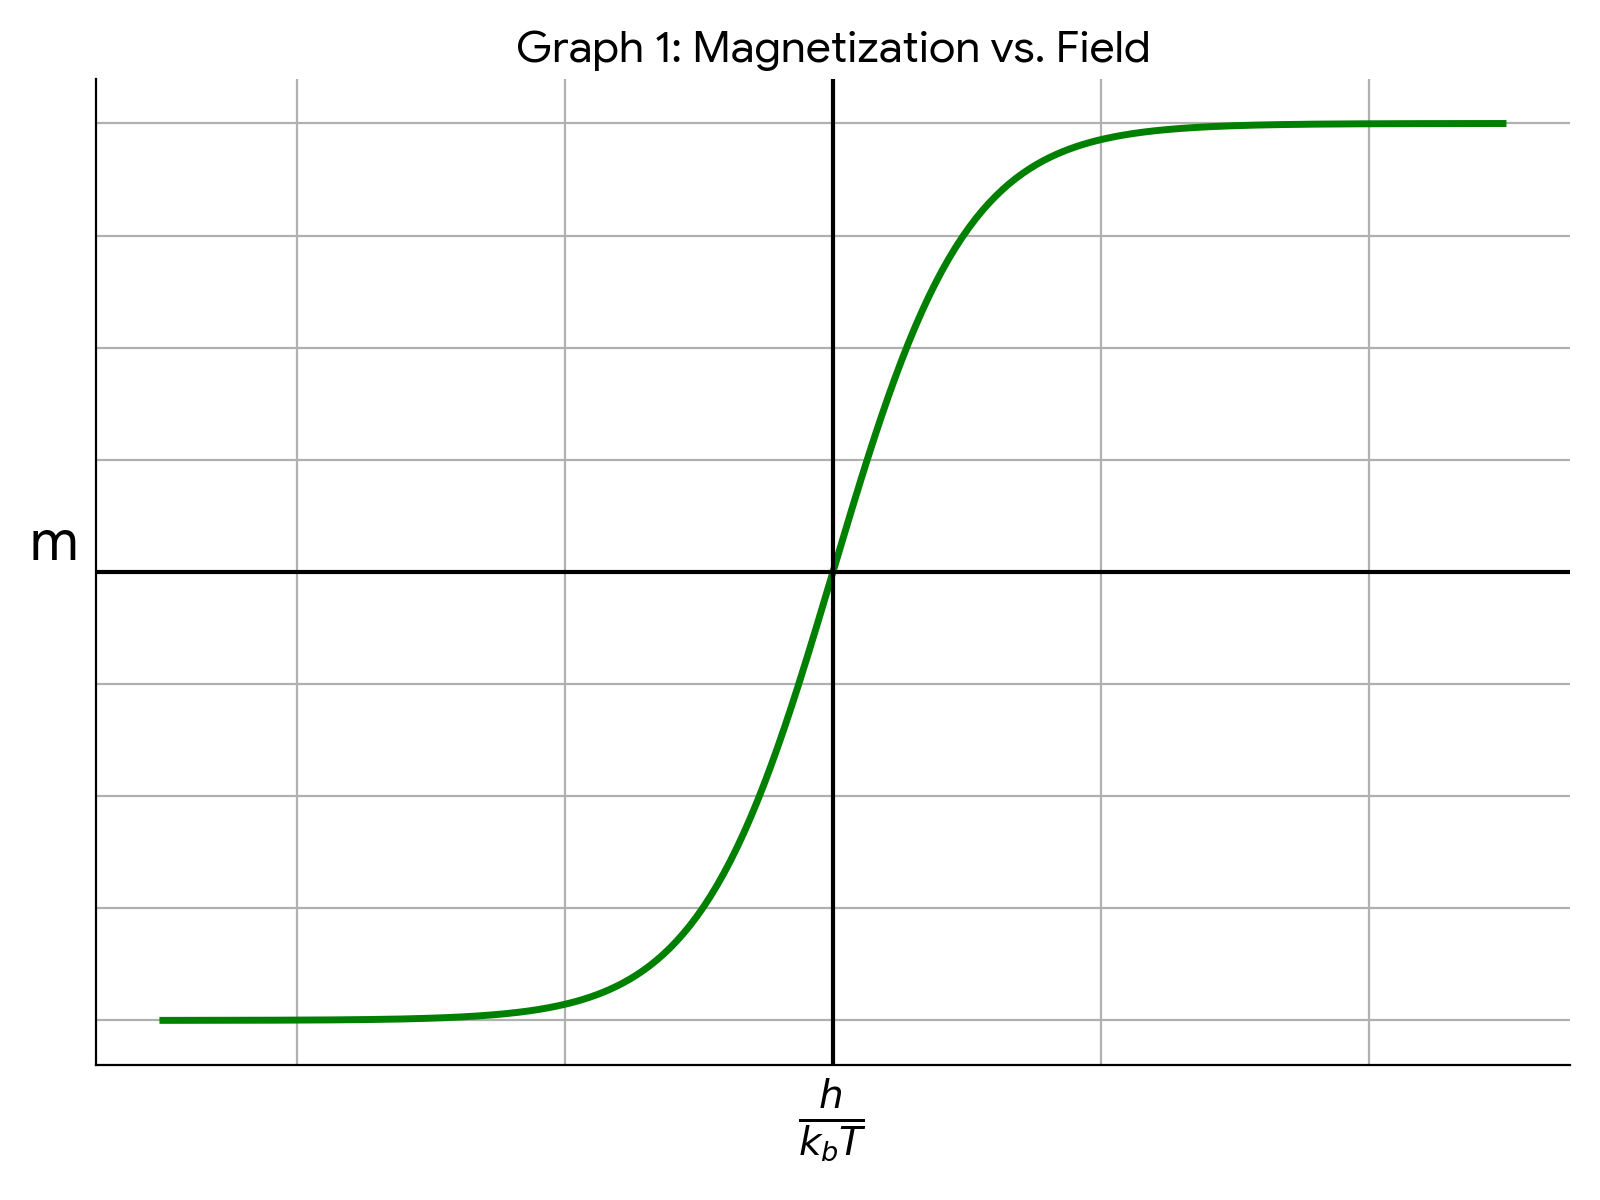
\includegraphics[width=0.6\textwidth]{pics/17_1.png} % INSERIRE QUI IL PERCORSO DEL GRAFICO
\caption{Andamento della magnetizzazione $m$ in funzione di $\beta h$ per $J=0$.}
\label{fig:ch17_1}
\end{figure}

\subsection*{Caso 2: $h = 0$, $J > 0$ (Interazioni senza Campo Esterno)}
Risolviamo l'equazione graficamente. Cerchiamo le intersezioni tra le due curve:
\begin{itemize}
    \item $y_1 = m$ (una retta con pendenza 1)
    \item $y_2 = \tanh(\beta z J m)$ (una tangente iperbolica)
\end{itemize}

La pendenza della tangente iperbolica nell'origine ($m=0$) è $\beta z J$. Il comportamento del sistema dipende dal confronto tra questa pendenza e la pendenza di $y_1$.

\subsubsection*{Alta Temperatura: $T > T_c$}
Se la temperatura è alta, $\beta$ è piccolo, quindi $\beta z J < 1$.
La pendenza della tangente iperbolica all'origine è minore di 1.
C'è solo un'intersezione in $m=0$. La magnetizzazione di equilibrio è nulla; il sistema è disordinato perché il rumore termico domina sull'interazione.

\begin{figure}[h!]
\centering
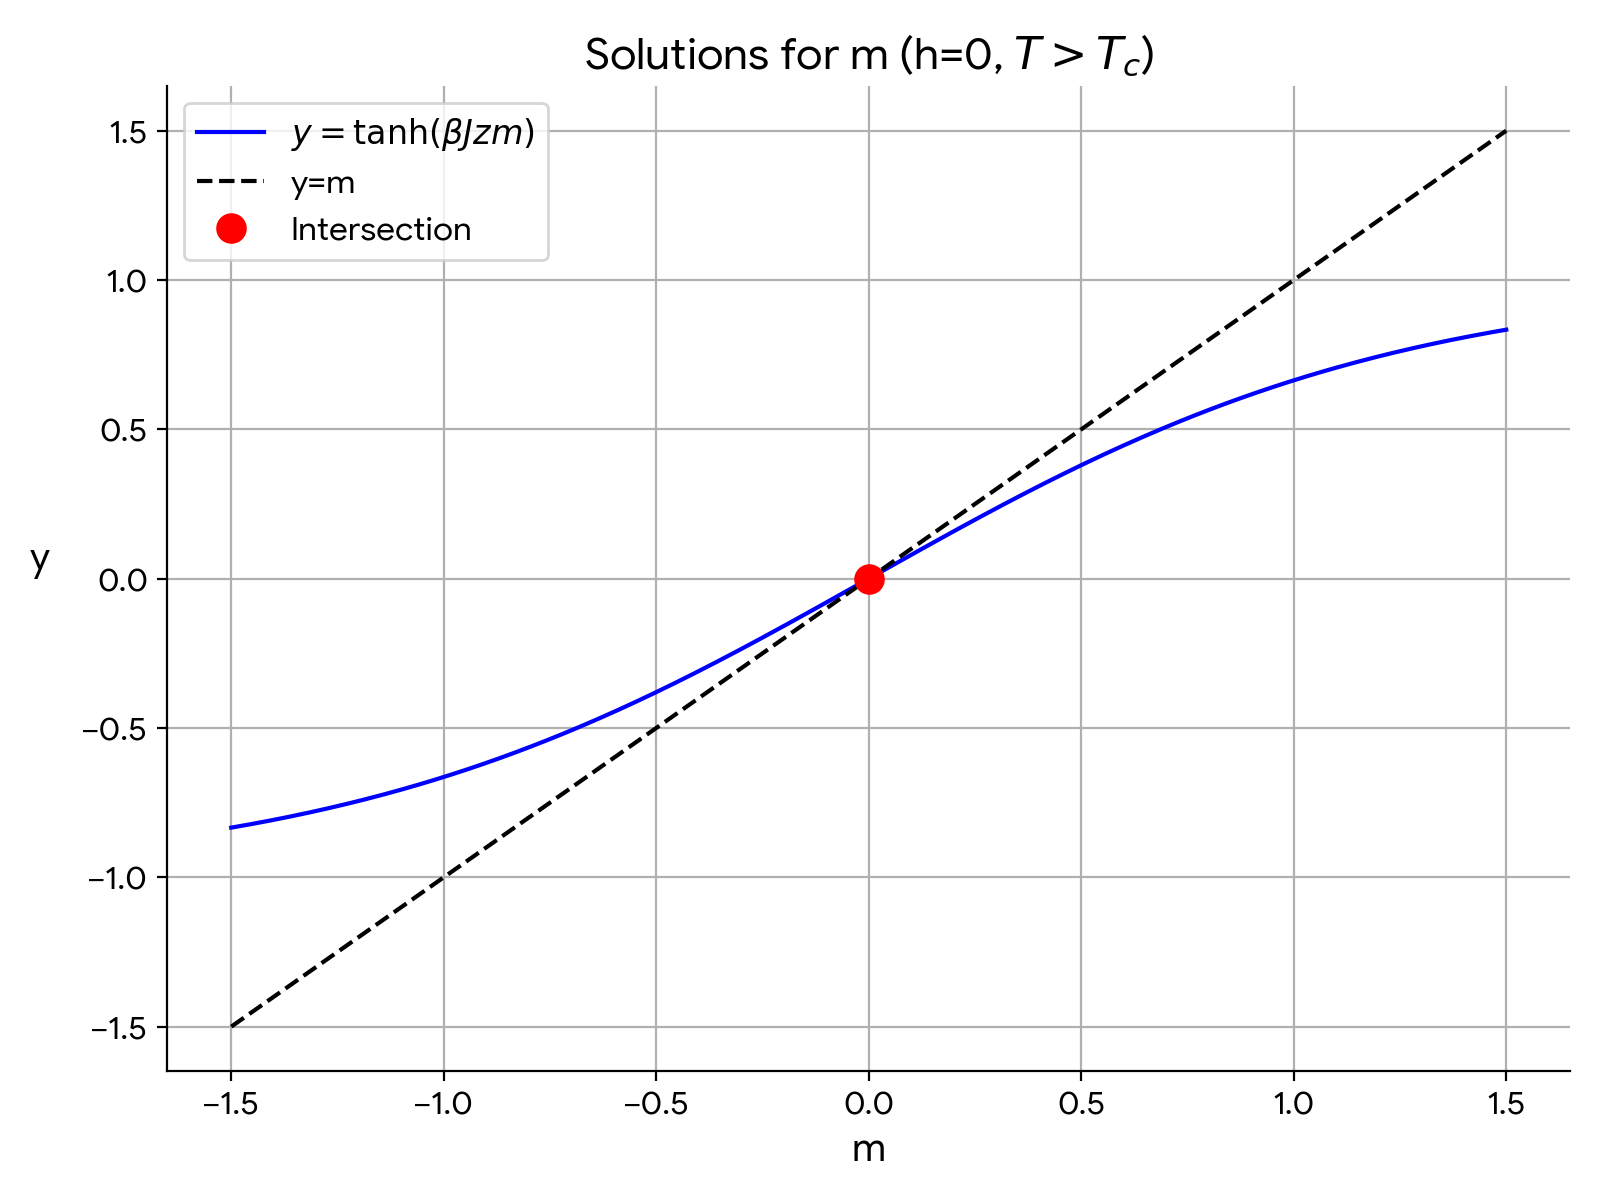
\includegraphics[width=0.6\textwidth]{pics/17_2.png} % INSERIRE QUI IL PERCORSO DEL GRAFICO
\caption{Soluzione per $T > T_c$.}
\label{fig:ch17_2}
\end{figure}

\subsubsection*{Temperatura Critica: $T = T_c$}
Esiste una temperatura critica $T_c$ tale che $\beta_c z J = 1$. Questo definisce la temperatura critica:

\begin{equation} \label{eq:ch17_12}
T_c = \frac{zJ}{k_B}
\end{equation}

A $T=T_c$, la pendenza della tangente iperbolica all'origine è esattamente 1. Anche in questo caso, l'unica soluzione è $m=0$.

\begin{figure}[h!]
\centering
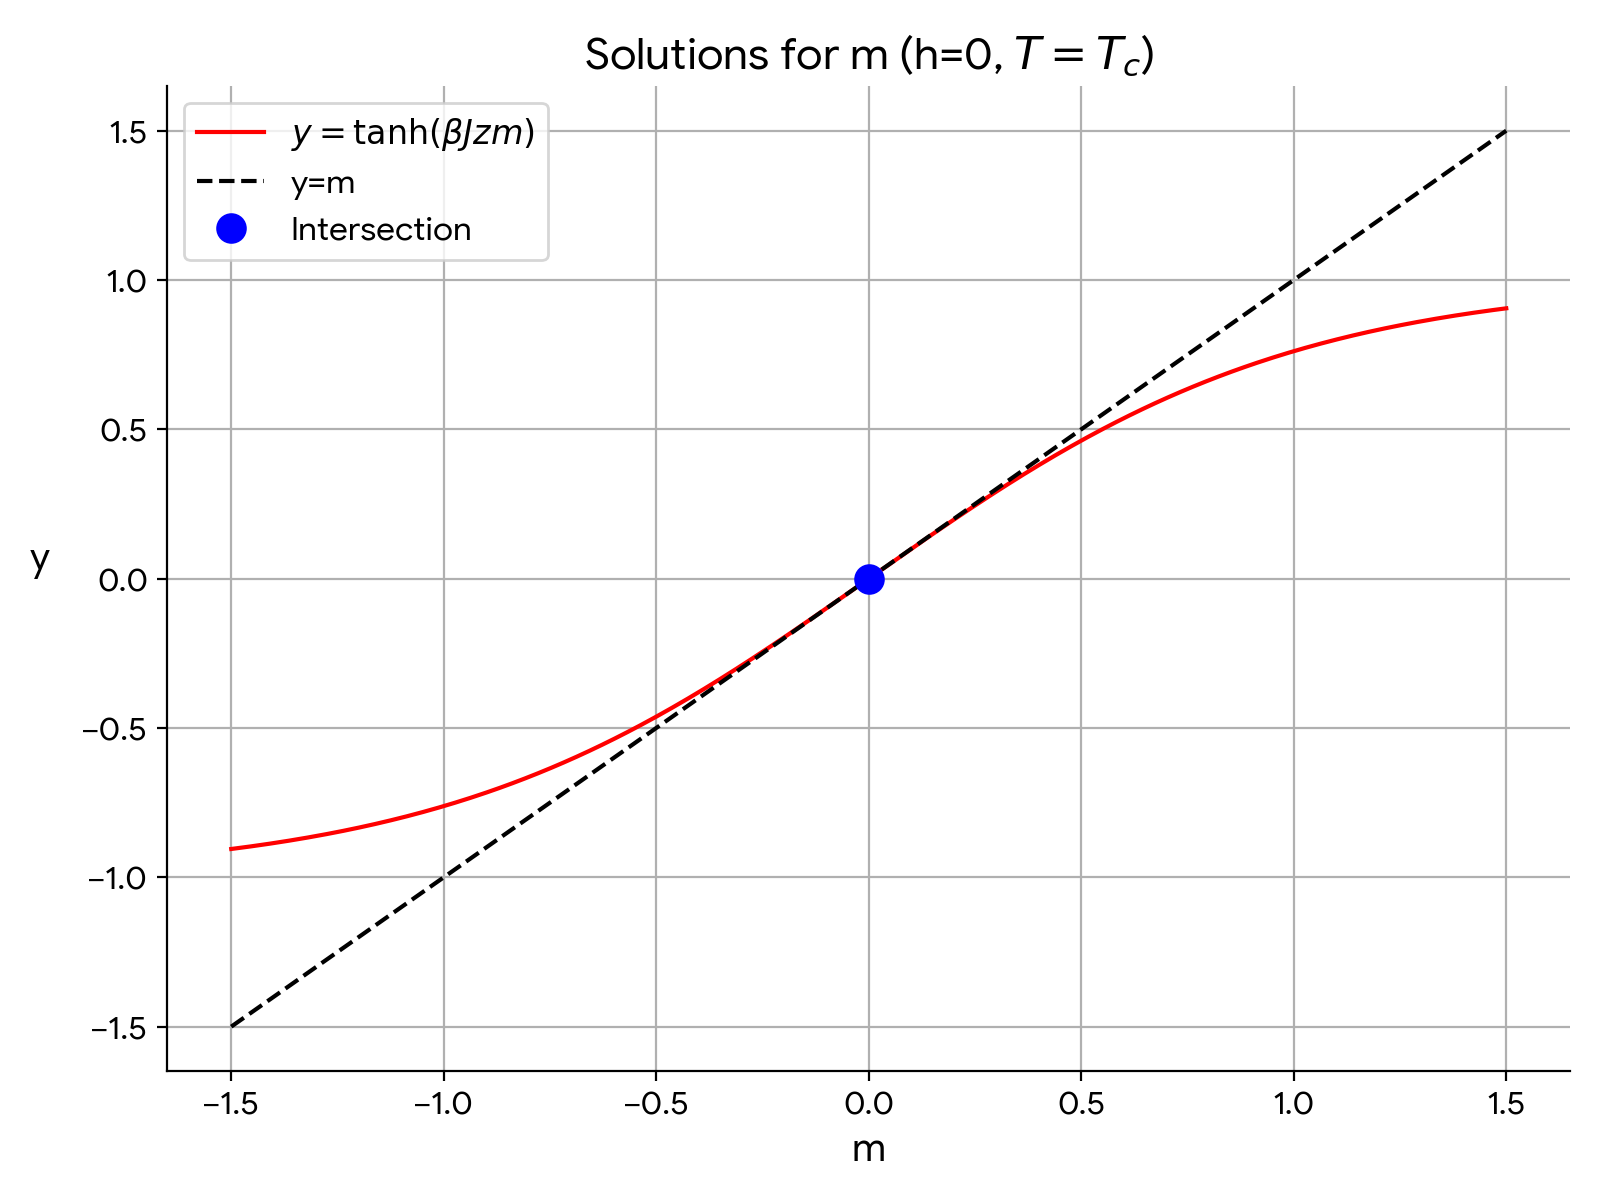
\includegraphics[width=0.6\textwidth]{pics/17_3.png} % INSERIRE QUI IL PERCORSO DEL GRAFICO
\caption{Soluzione per $T = T_c$.}
\label{fig:ch17_3}
\end{figure}

\subsubsection*{Bassa Temperatura: $T < T_c$}
Se $T < T_c$, allora $\beta z J > 1$. La pendenza della tangente iperbolica all'origine è maggiore di 1.
In questo caso, oltre alla soluzione $m=0$, compaiono altre due soluzioni simmetriche, $m^+$ e $m^-$.
La soluzione $m=0$ è instabile, mentre le soluzioni $m^\pm$ sono stabili. Il sistema sceglie spontaneamente una di queste due magnetizzazioni non nulle.

\begin{figure}[h!]
\centering
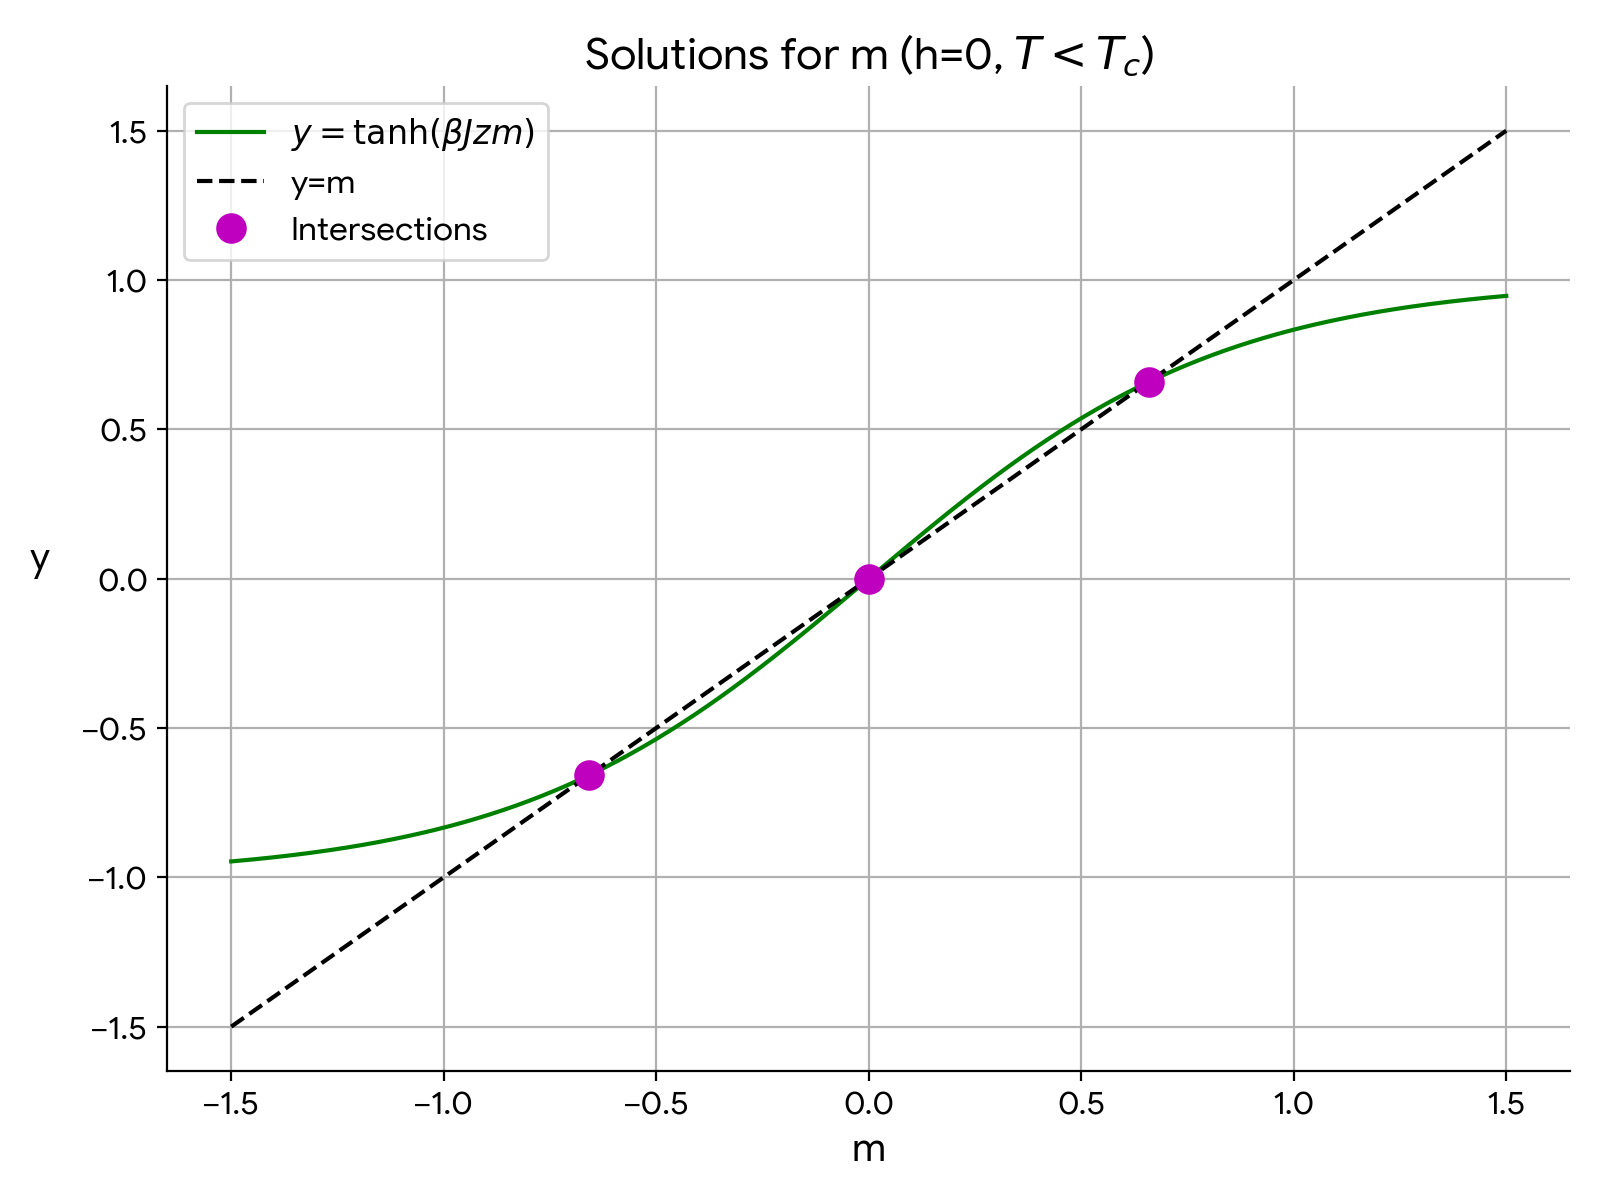
\includegraphics[width=0.6\textwidth]{pics/17_4.png} % INSERIRE QUI IL PERCORSO DEL GRAFICO
\caption{Soluzione per $T < T_c$.}
\label{fig:ch17_4}
\end{figure}

Il diagramma di $m$ in funzione di $T$ mostra che per $T>T_c$, $m=0$. A $T=T_c$, la soluzione si biforca, e per $T<T_c$ appaiono due rami di soluzioni stabili $m^\pm$.

\begin{figure}[h!]
\centering
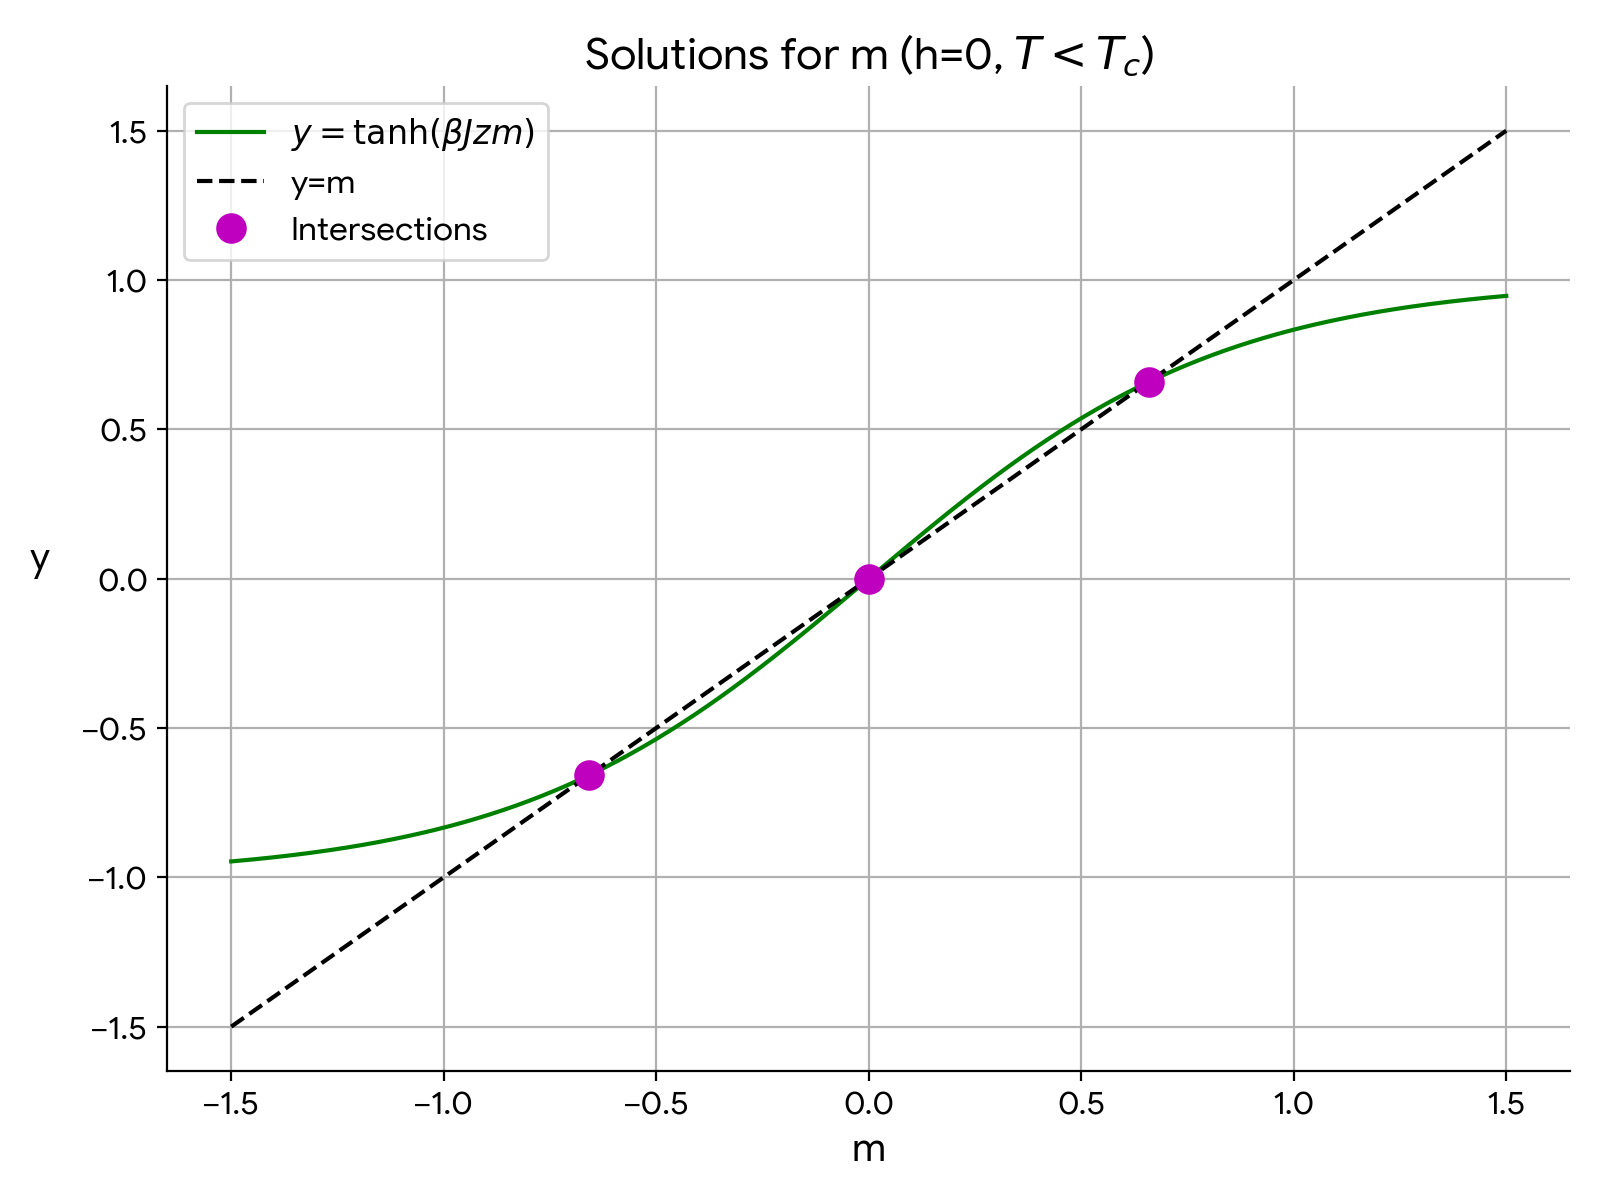
\includegraphics[width=0.6\textwidth]{pics/17_4.png} % INSERIRE QUI IL PERCORSO DEL GRAFICO DELLA BIFORCAZIONE
\caption{Diagramma di biforcazione della magnetizzazione $m$ in funzione della temperatura $T$.}
\label{fig:ch17_5}
\end{figure}


\section{Dalla Magnetizzazione alla Distribuzione di Probabilità}
La soluzione dell'equazione di autoconsistenza fornisce la magnetizzazione di equilibrio $m_{eq}$, ovvero il valore che misureremmo in un esperimento macroscopico. Tuttavia, su scale di tempo microscopiche, la magnetizzazione istantanea $m = \frac{1}{N} \sum_i S_i$ fluttua.
Vogliamo calcolare la distribuzione di probabilità $P(m)$ per questi valori istantanei.

Formalmente, si calcola sommando le probabilità di tutte le microconfigurazioni $\{S_i\}$ che corrispondono a un dato valore di $m$:

\begin{equation} \label{eq:ch17_13}
P\left(m = \frac{1}{N}\sum_i s_i\right) = \sum_{\{s_i\}} P(\{s_i\}) \delta\left(m - \frac{1}{N}\sum_i s_i\right)
\end{equation}

Sostituendo la probabilità di campo medio $P(\{s_i\}) \propto e^{-\beta H_{mf}}$ e usando la delta di Dirac per sostituire $\sum_i s_i = Nm$, l'espressione diventa:

\begin{equation} \label{eq:ch17_14}
P(m) = \frac{1}{Z_{TOT}} \sum_{\{s_i\}} e^{\beta h^{eff} (Nm) - \beta \frac{J N z m^2}{2}} \delta\left(m - \frac{1}{N}\sum_i s_i\right)
\end{equation}

L'obiettivo è scrivere questa probabilità nella forma $P(m) \propto e^{-\beta N f_{eff}(m)}$, dove $f_{eff}(m)$ è un'energia libera efficace. Per farlo, dobbiamo calcolare il termine entropico, ovvero la somma $\sum_{\{s_i\}} \delta(\dots)$, che conta il numero di configurazioni con magnetizzazione $m$.

Introduciamo il numero di spin "up" ($N^+$) e "down" ($N^-$):

\begin{equation} \label{eq:ch17_15}
M = \sum_i s_i = Nm = N^+ - N^-
\end{equation}
\begin{equation} \label{eq:ch17_16}
N = N^+ + N^-
\end{equation}

Risolvendo per $N^+$ e $N^-$:

\begin{equation} \label{eq:ch17_17}
N^+ = \frac{N(m+1)}{2} \quad , \quad N^- = \frac{N(1-m)}{2}
\end{equation}

Il numero di modi per arrangiare $N^+$ spin up e $N^-$ spin down su $N$ siti è dato dal coefficiente binomiale $\binom{N}{N^+}$. Usando l'approssimazione di Stirling ($\ln k! \approx k \ln k - k$) per $N$ grande, il suo logaritmo è:

\begin{equation} \label{eq:ch17_18}
\ln \binom{N}{N^+} = \ln N! - \ln N^+! - \ln N^-! \approx N\ln N - N^+\ln N^+ - N^-\ln N^-
\end{equation}

Sostituendo il termine entropico (espresso come $e^{\ln \binom{N}{N^+}}$) in $P(m)$, l'esponente completo diventa:

\begin{equation} \label{eq:ch17_19}
N\beta h^{eff}m - \beta \frac{J N z m^2}{2} + N\ln N - N^+\ln N^+ - N^-\ln N^-
\end{equation}

Sostituendo le espressioni di $N^+$ e $N^-$ in funzione di $m$ nei termini logaritmici e semplificando, i termini in $N\ln N$ si cancellano e l'esponente diventa:

\begin{equation*}
N\beta h^{eff}m - \beta \frac{J N z m^2}{2} - N\frac{1+m}{2}\ln(1+m) - N\frac{1-m}{2}\ln(1-m) + N\ln 2
\end{equation*}

Raccogliamo ora un fattore $-\beta N$ per identificare l'energia libera efficace $f_{eff}(m)$:

\begin{align} \label{eq:ch17_20}
P(m) &\propto \frac{1}{\mathcal{N}}\exp \left\{ -\beta N \left[ -mh^{eff} + \frac{J z m^2}{2} \right. \right. \nonumber\\ &\left. \left. + \frac{k_B T}{2} \left( (1+m)\ln(1+m) + (1-m)\ln(1-m) - 2\ln 2 \right) \right] \right\}
\end{align}

L'energia libera efficace per spin $f_{eff}(m)$ è l'espressione tra parentesi quadre. Trascurando la costante $-k_B T \ln 2$ (che viene assorbita nella normalizzazione), otteniamo:

\vspace{0.5cm}
\noindent\fbox{%
    \parbox{\dimexpr\linewidth-2\fboxsep-2\fboxrule\relax}{%
        \begin{equation*}
        f_{eff}(m) = -mh^{eff} + \frac{Jzm^2}{2} + \frac{k_B T}{2} [(1+m)\ln(1+m) + (1-m)\ln(1-m)]
        \end{equation*}
    }%
}
\vspace{0.5cm}


\section{Interpretazione di $f_{eff}(m)$}
Il valore di equilibrio della magnetizzazione, $m_{eq}$, corrisponde al valore $m^*$ che massimizza la probabilità $P(m)$. Per $N$ grande (metodo di Laplace), questo equivale a trovare il valore di $m$ che minimizza l'energia libera efficace $f_{eff}(m)$. Per trovare i minimi, poniamo la derivata uguale a zero:

\begin{equation} \label{eq:ch17_21}
\frac{d}{dm}f_{eff}(m) = 0
\end{equation}

Svolgendo la derivata, si ritrova esattamente l'equazione di autoconsistenza, mostrando la coerenza dell'approccio:

\begin{equation} \label{eq:ch17_22}
m = \tanh(\beta h_{eff}) = \tanh(\beta h + \beta z J m)
\end{equation}

L'analisi di $f_{eff}(m)$ conferma i risultati della soluzione grafica e permette di determinare la stabilità delle soluzioni.
Per $h=0$:
\begin{itemize}
    \item \textbf{$T > T_c$}: $f_{eff}(m)$ ha un solo minimo in $m=0$.
    \begin{figure}[h!]
\centering
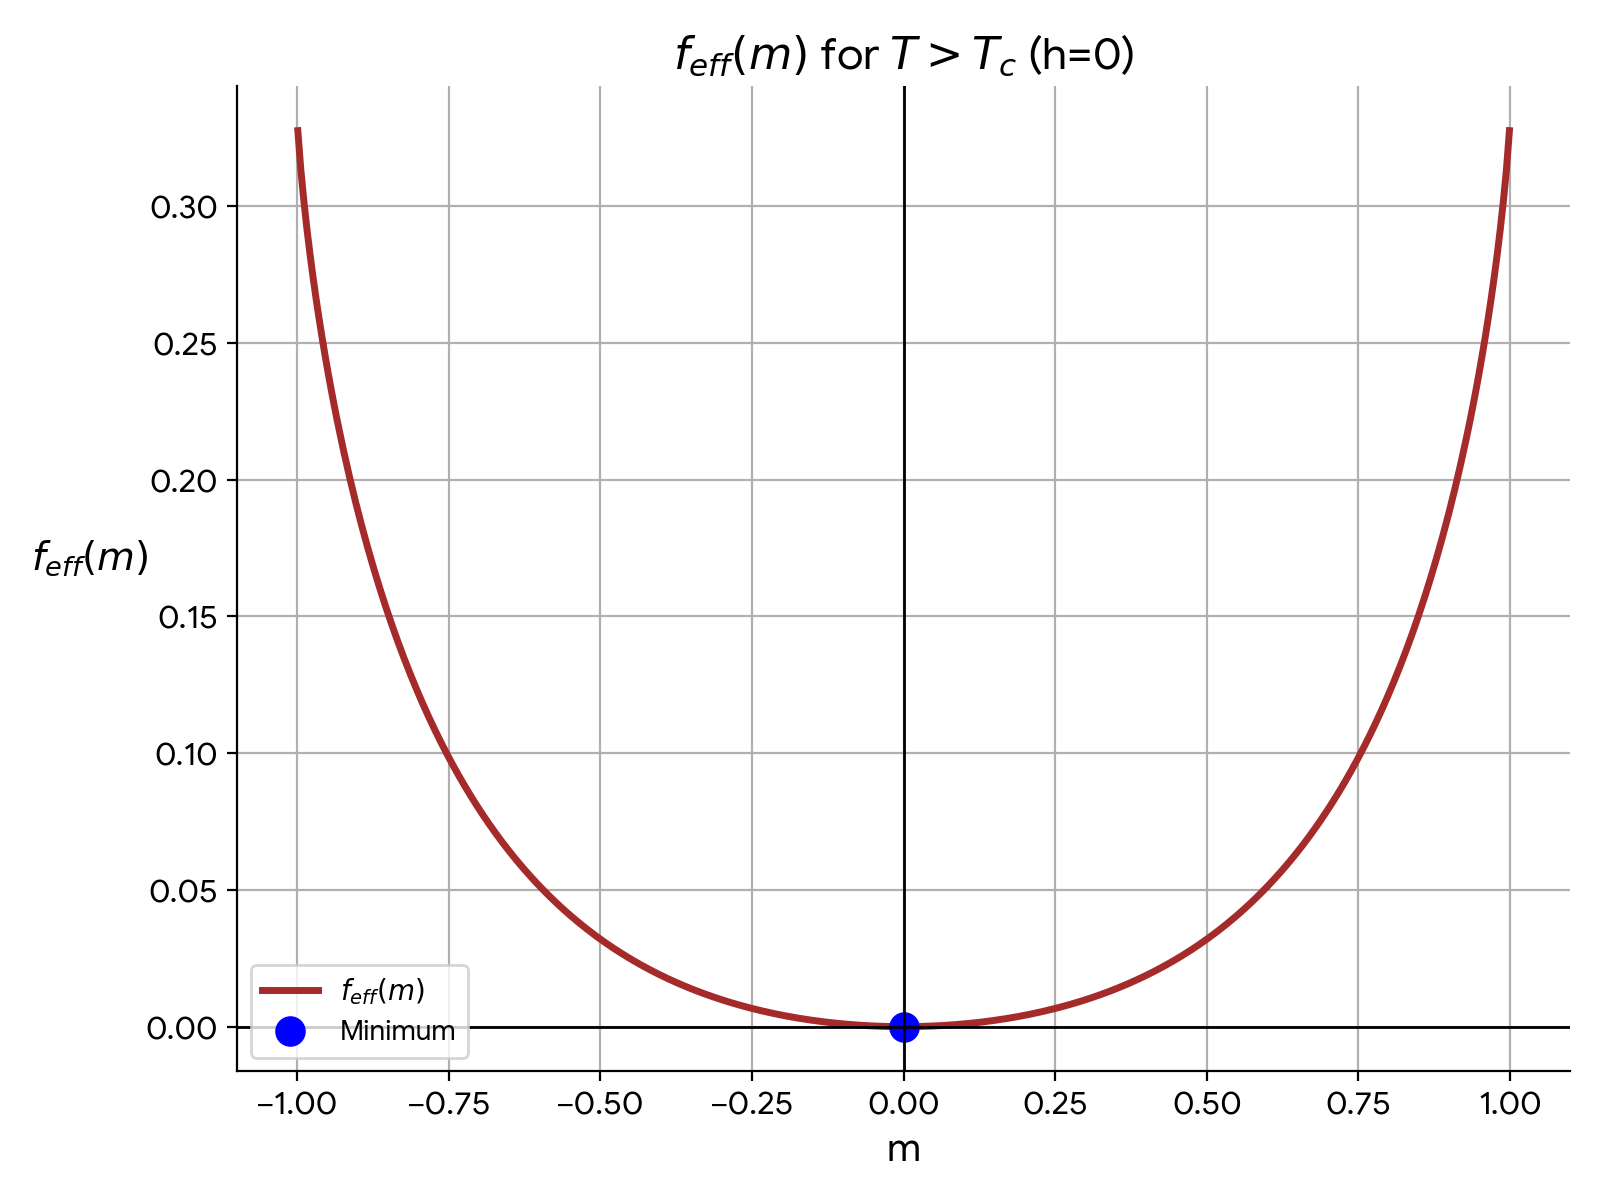
\includegraphics[width=0.6\textwidth]{pics/17_6.png} % INSERIRE QUI IL PERCORSO DEL GRAFICO DELLA DOPPIA BUCA
\caption{Profilo dell'energia libera efficace $f_{eff}(m)$ per $T > T_c$.}
\label{fig:ch17_6}
\end{figure}
    \item \textbf{$T = T_c$}: Il minimo in $m=0$ diventa molto piatto. Sia la derivata prima che la derivata seconda sono zero in $m=0$. Una derivata seconda nulla è associata a una suscettibilità magnetica divergente, $\chi = \frac{dm}{dh}\Big|_{h=0} \to \infty$, che è un segno distintivo di una transizione di fase continua (del secondo ordine).
     \begin{figure}[h!]
\centering
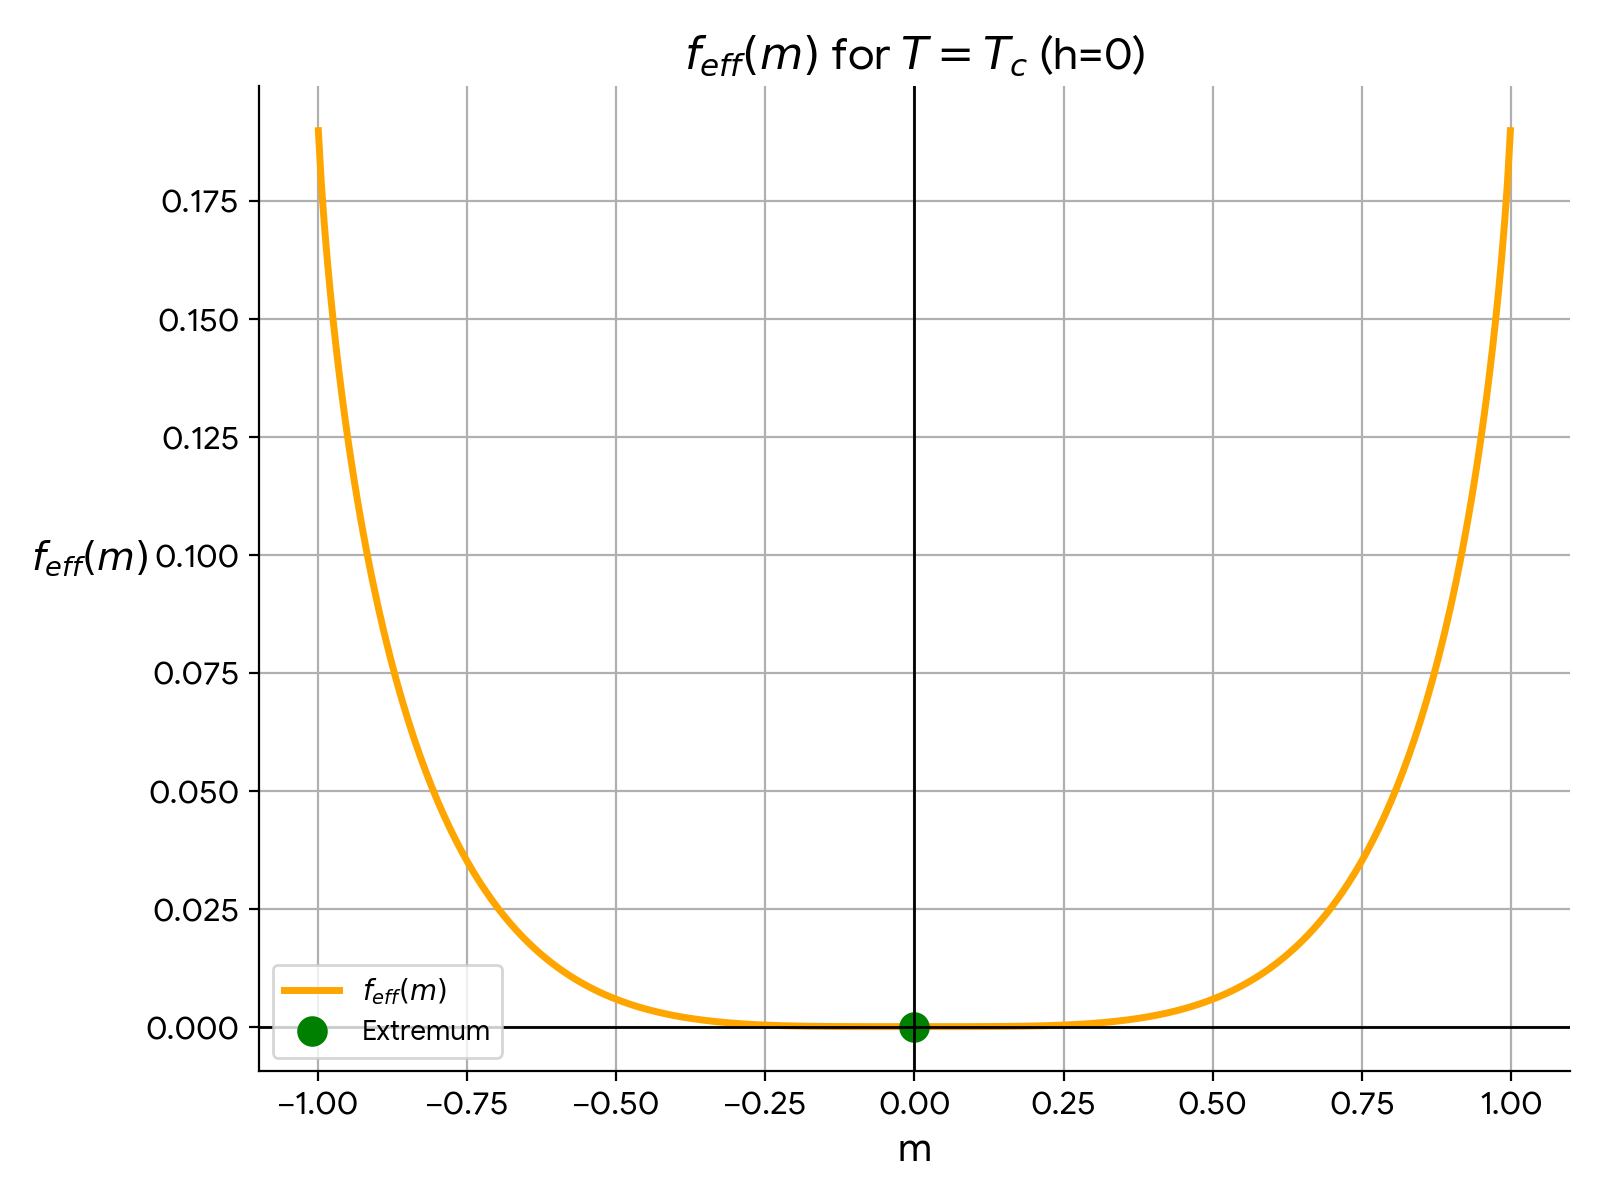
\includegraphics[width=0.6\textwidth]{pics/17_7.png} % INSERIRE QUI IL PERCORSO DEL GRAFICO DELLA DOPPIA BUCA
\caption{Profilo dell'energia libera efficace $f_{eff}(m)$ per $T = T_c$.}
\label{fig:ch17_7}
\end{figure}
    \item \textbf{$T < T_c$}: La forma della funzione cambia in una "doppia buca" (double well). Ci sono due minimi simmetrici in $m^\pm$, che sono le soluzioni stabili. Il punto $m=0$ è ora un massimo locale, che corrisponde a una soluzione instabile.
 \begin{figure}[h!]
\centering
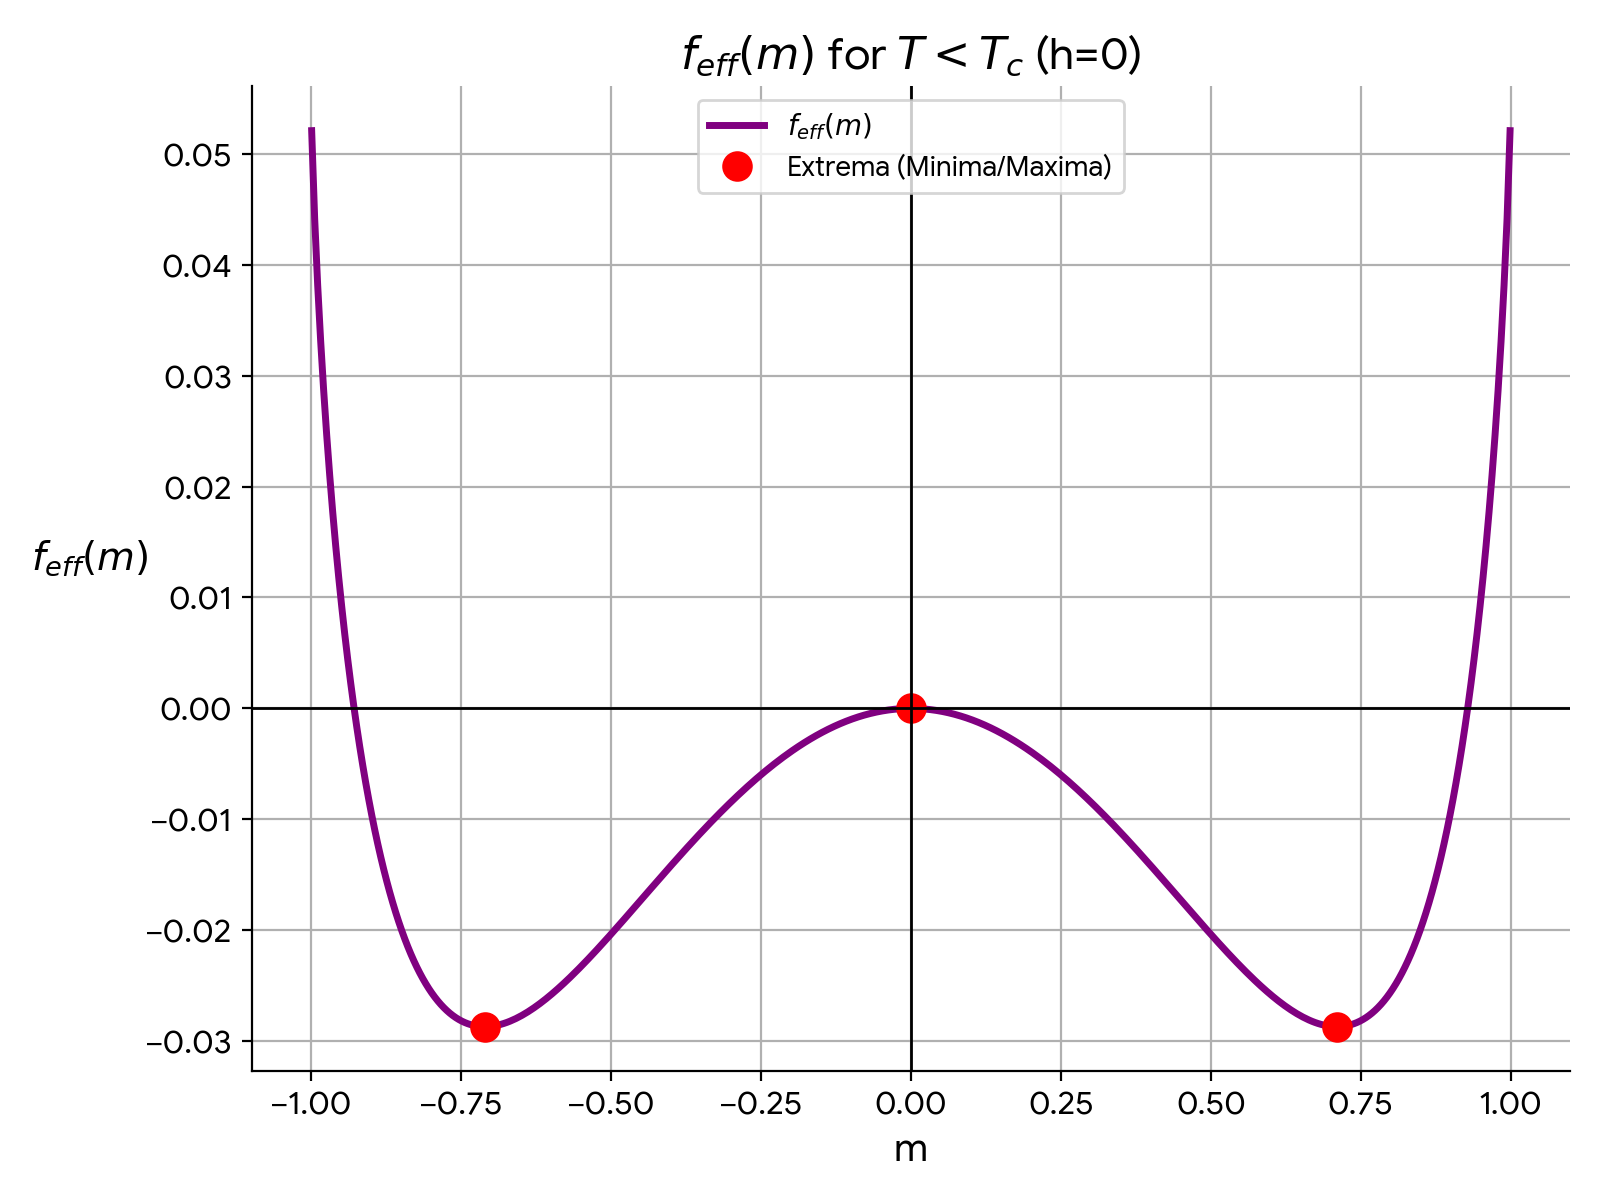
\includegraphics[width=0.6\textwidth]{pics/17_8.png} % INSERIRE QUI IL PERCORSO DEL GRAFICO DELLA DOPPIA BUCA
\caption{Profilo dell'energia libera efficace $f_{eff}(m)$ per $T < T_c$.}
\label{fig:ch17_8}
\end{figure}
\end{itemize}



\subsection*{Caso: $T > T_c$ e $h > 0$}
Consideriamo ora cosa accade quando viene applicato un campo esterno. Esaminiamo il caso ad alta temperatura in presenza di un campo positivo.

Dobbiamo risolvere $m = \tanh(\beta h + \beta z J m)$. La retta $y=m$ non cambia. La curva della tangente iperbolica, invece, è traslata. Il suo argomento si annulla non più in $m=0$, ma quando:

\begin{equation} \label{eq:ch17_23}
\beta h + \beta z J m = 0 \implies m_0 = -\frac{h}{zJ}
\end{equation}

Poiché siamo nel regime $T > T_c$, la pendenza della tangente iperbolica è sempre minore di 1.
Di conseguenza, la curva traslata interseca la retta $y=m$ in un solo punto, che corrisponde a un valore di magnetizzazione $m_{eq} > 0$. La magnetizzazione di equilibrio è sempre positiva se il campo è positivo. Il comportamento qualitativo di $m$ in funzione di $h$ è simile a quello del caso non interagente.

 \begin{figure}[h!]
\centering
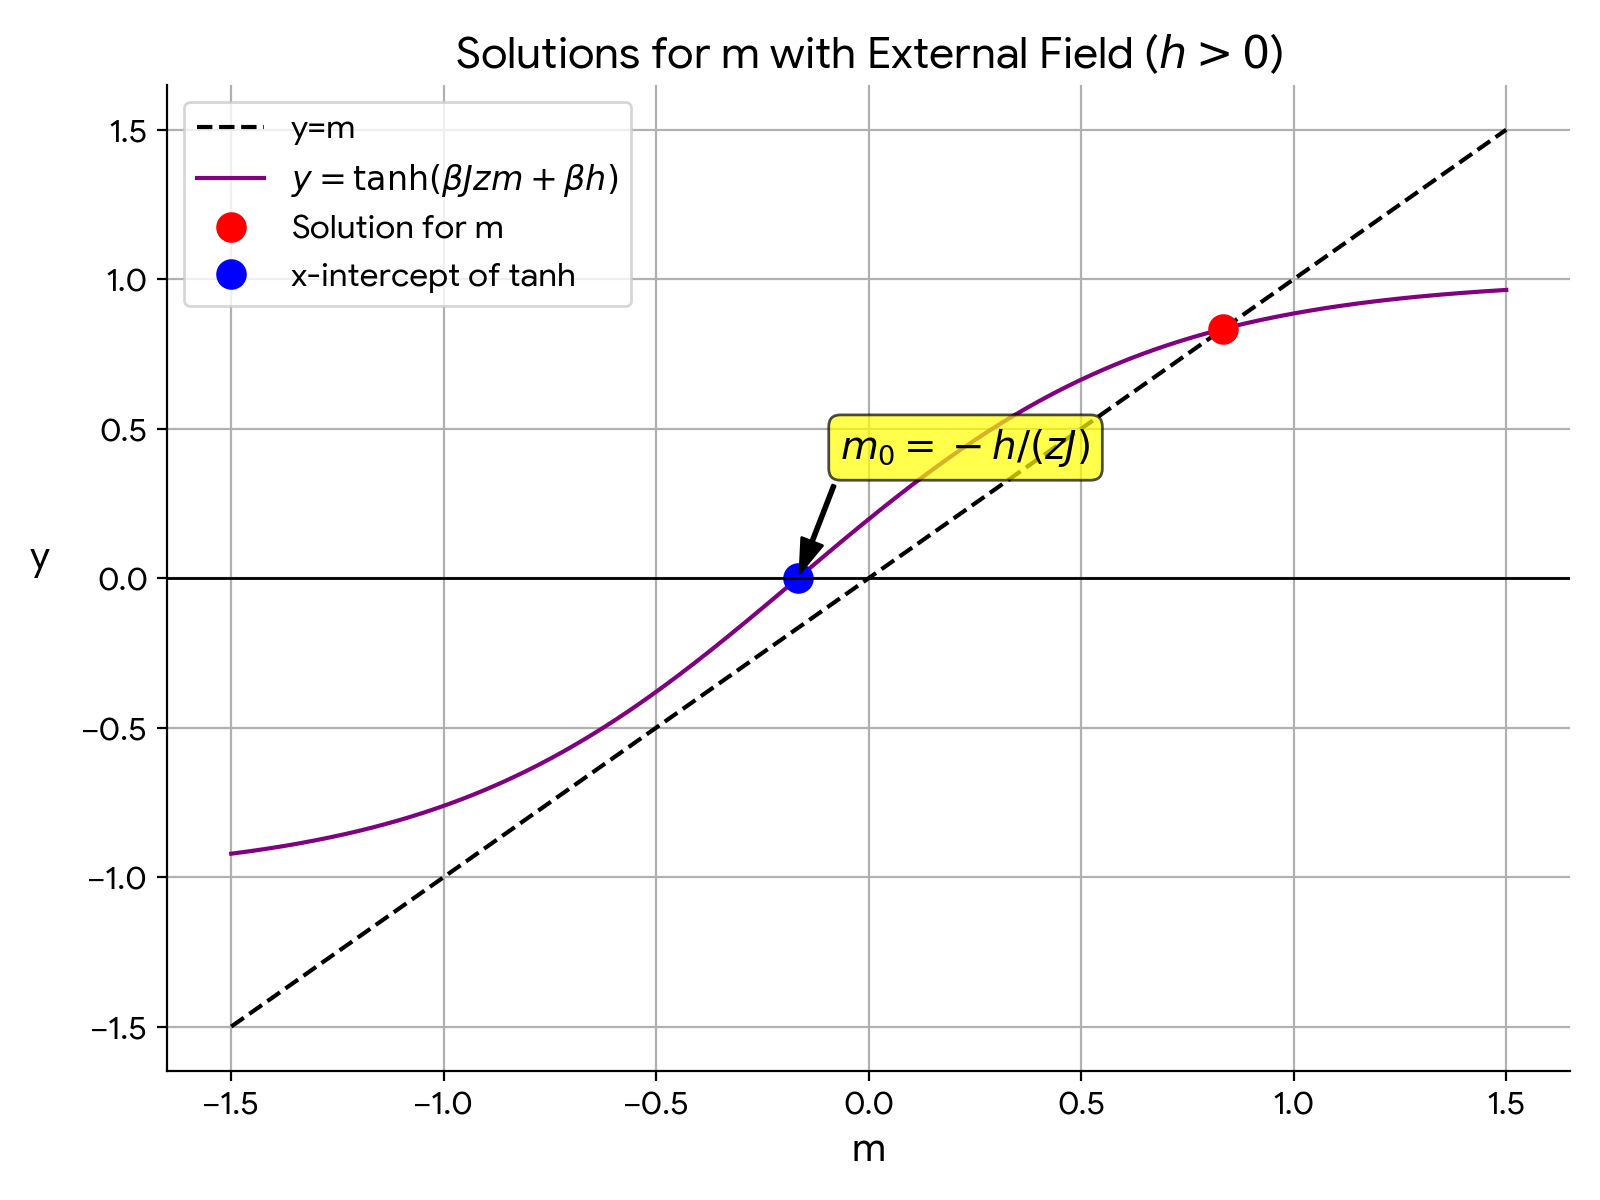
\includegraphics[width=0.6\textwidth]{pics/17_9.png} % INSERIRE QUI IL PERCORSO DEL GRAFICO DELLA DOPPIA BUCA
\caption{Soluzione grafica per $h > 0$.}
\label{fig:ch17_9}
\end{figure}

In questo stesso regime ($T > T_c$, $h>0$), la funzione di energia libera efficace $f_{eff}(m)$ presenta un singolo minimo. A causa del campo esterno, questo minimo non è più in $m=0$, ma è spostato sull'asse positivo, in corrispondenza del valore $m_{eq}$ trovato con il metodo grafico. Questo conferma che c'è un unico stato di equilibrio stabile con magnetizzazione positiva.

\begin{figure}[h!]
\centering
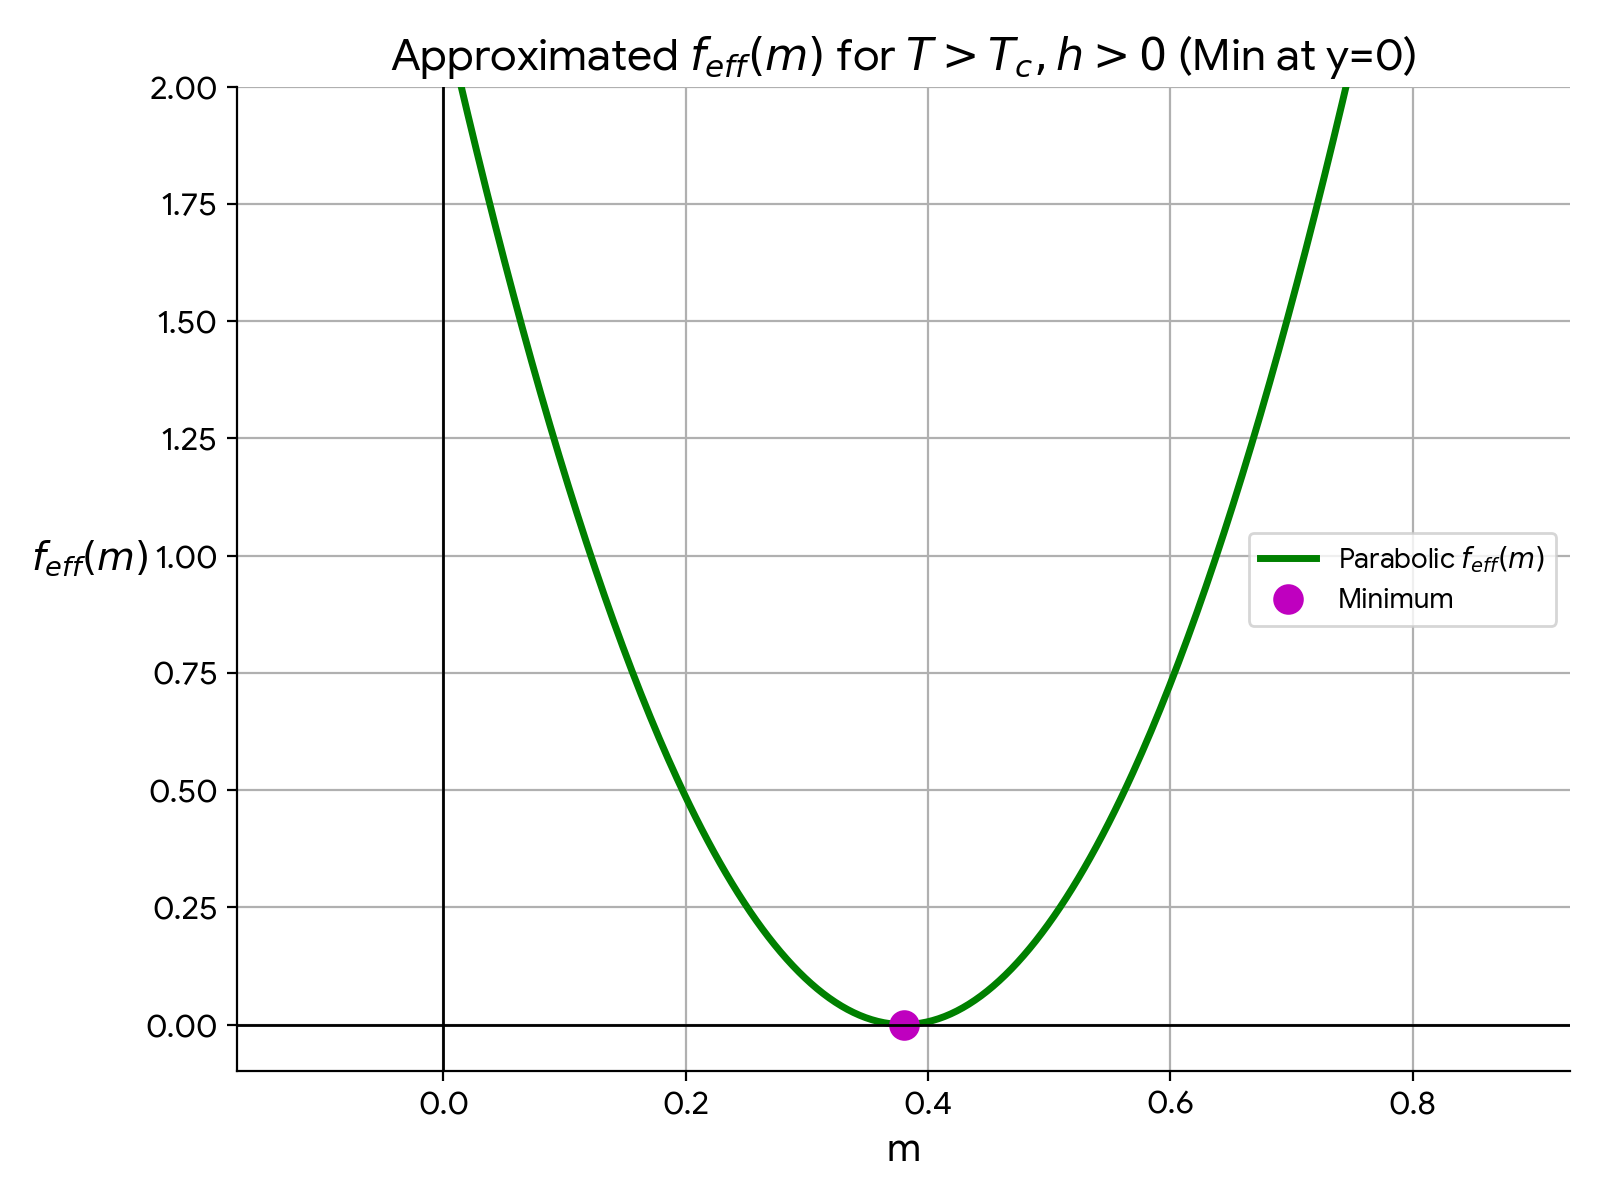
\includegraphics[width=0.6\textwidth]{pics/17_10.png} % INSERIRE QUI IL PERCORSO DEL GRAFICO CON CAMPO ESTERNO
\caption{Energia libera efficace $f_{eff}(m)$ nel caso $T > T_c$ e $h > 0$.}
\label{fig:ch17_10}
\end{figure}



